%%%%%%%%%%%%%%%%%%%%%%%%%%%

%%%%%%%%%%%%%%%%%%%%%%%%%%%_________________CHAPTERFOUR_________________%%%%%%%%%%%%%%%%%%%%%%%%%%%

%%%%%%%%%%%%%%%%%%%%%%%%%%%

\chapter{Chapter 4 Supplemental Information}
\label{sec:app4}
\clearpage
\section{Supplemental Figures}

%Supplemental Figure 1: Chlorophyll values in experiments and in situ samples 
\begin{figure}[h!]
  \centering
    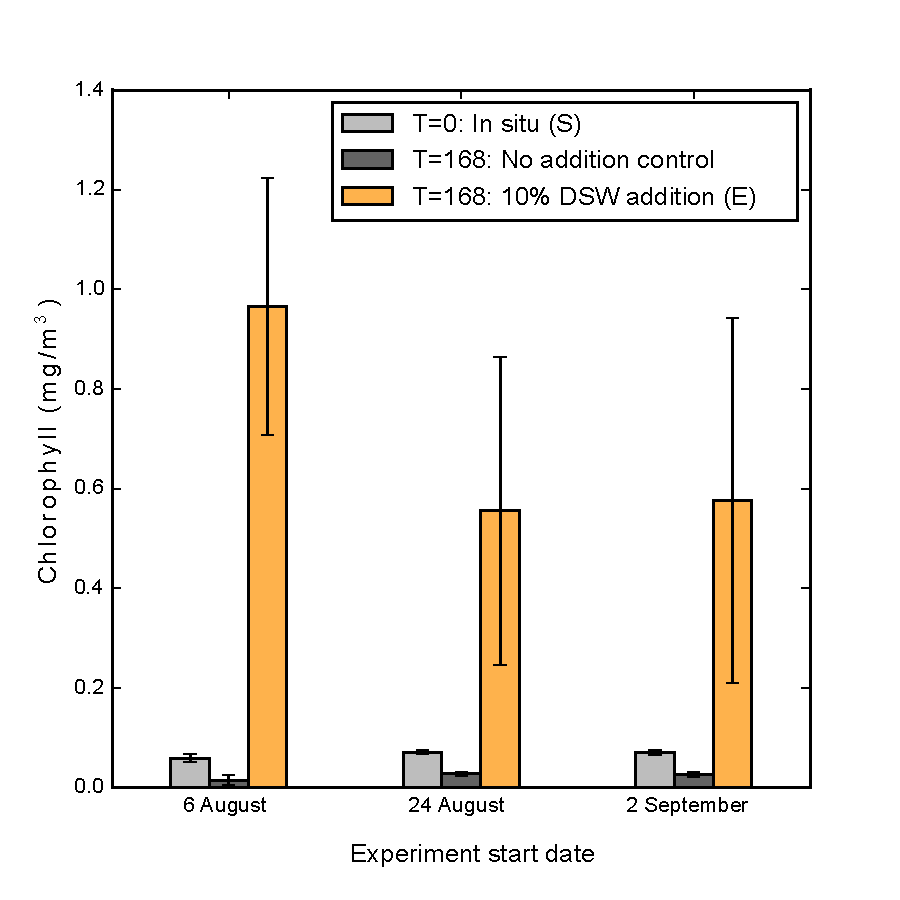
\includegraphics[width=1\textwidth]{Images/C4_FigureS1.pdf}
    \caption[Chlorophyll a of replicated experiments for \emph{in situ} samples, no addition control, and a 10\% deep seawater amendment]{Chlorophyll a of replicated experiments for \emph{in situ} samples (S), a no addition control, and a 10\% deep seawater (DSW) amendment (E). Incubation samples were harvested after 168 hours.}
  \label{fig:a4f1}
\end{figure}


%Supplemental Figure 2: Rank abundance shifts in species composition of diatoms, haptophytes and dinoflagellates

\begin{landscape}
 %  \null         %%<---- this is needed
   \vfill        %%<-----here
\begin{figure}[p!]
  \centering
    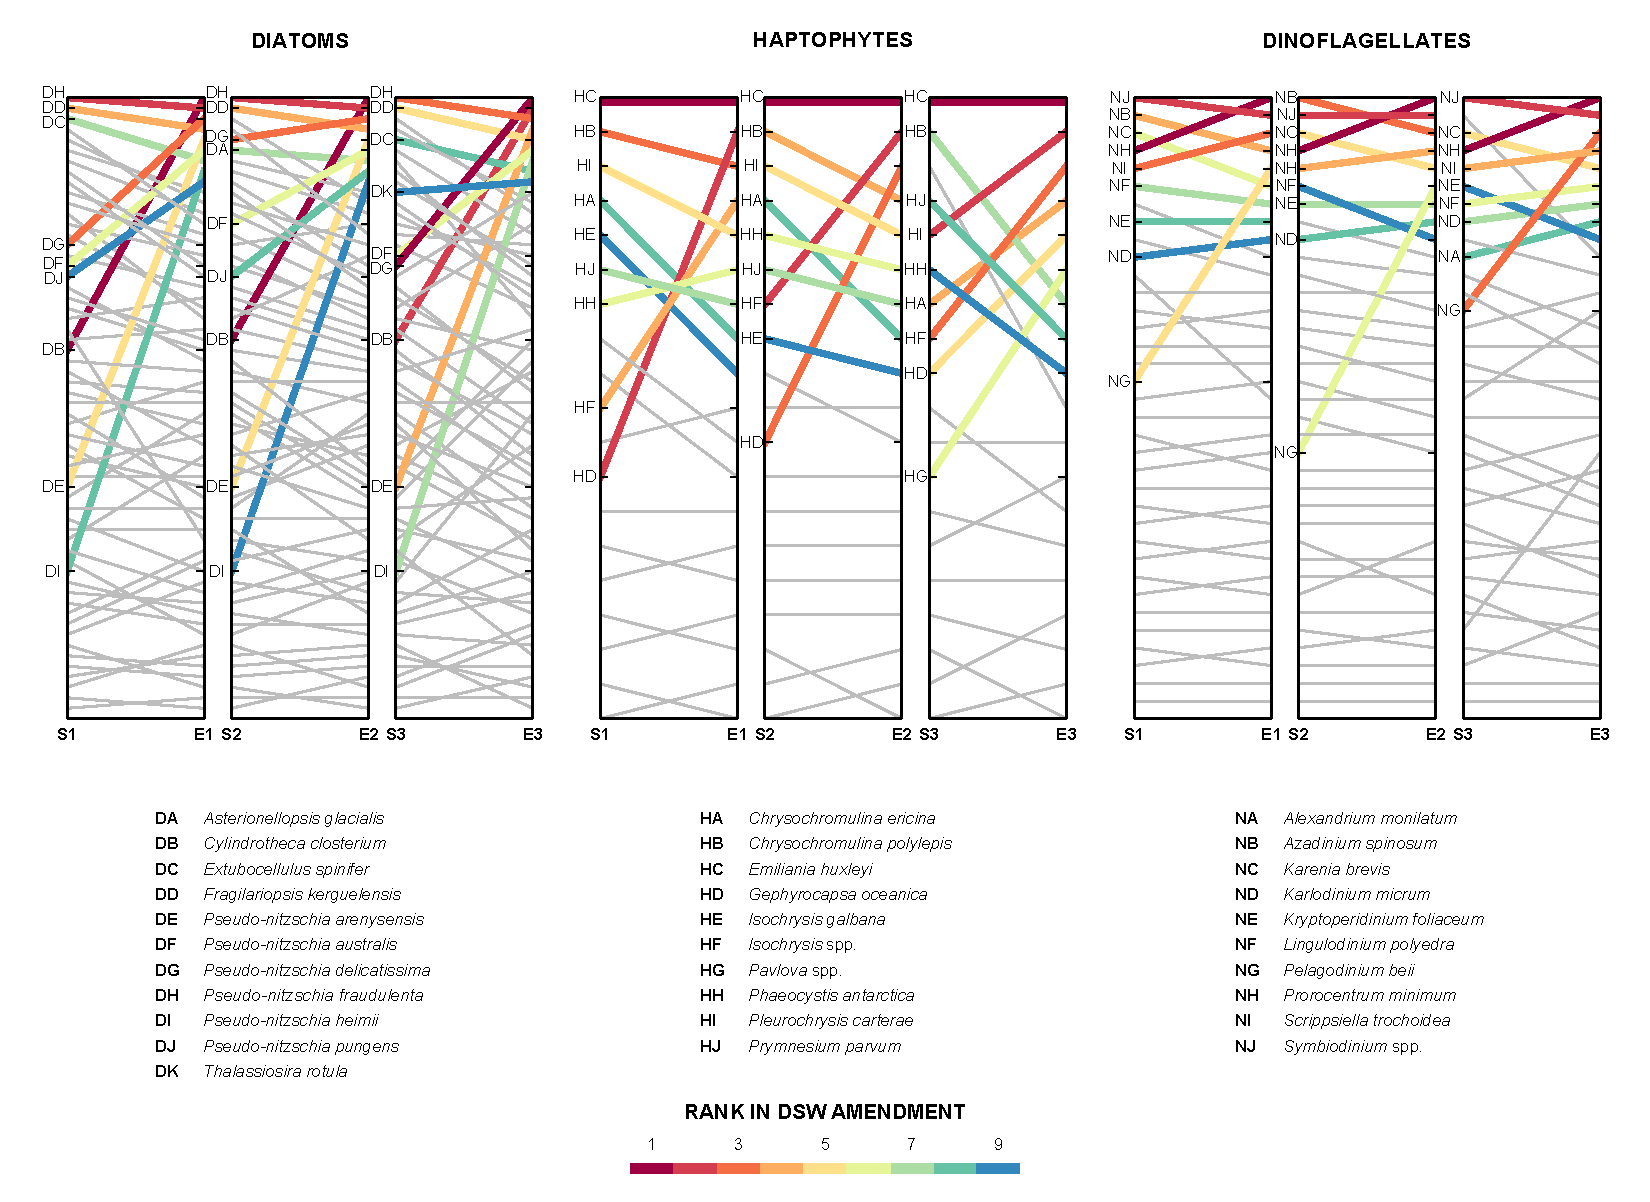
\includegraphics[width=1\textwidth]{Images/C4_FigureS2.pdf}
    \caption[Rank abundance shifts in the species composition of diatoms, haptophytes and dinoflagellates]{Rank abundance shifts in the species composition of diatoms, haptophytes and dinoflagellates for the three experiments. The relative shift in rank abundance for each species is depicted for each incubation experiment (E1-E3) following deep seawater (DSW) addition. The nine most abundant taxa following DSW addition are highlighted for each of the functional groups. Although the species that recruited the reads are denoted here this is highly driven by the composition of the database and does not necessarily indicate the actual species present, but rather the closest species present in the database.}
  \label{fig:a4f2}
\end{figure}
    \vfill        %%<----- and here
\end{landscape}


%Supplemental Figure 3: QMF Comparison across species


\begin{figure}[p!]
  \centering
    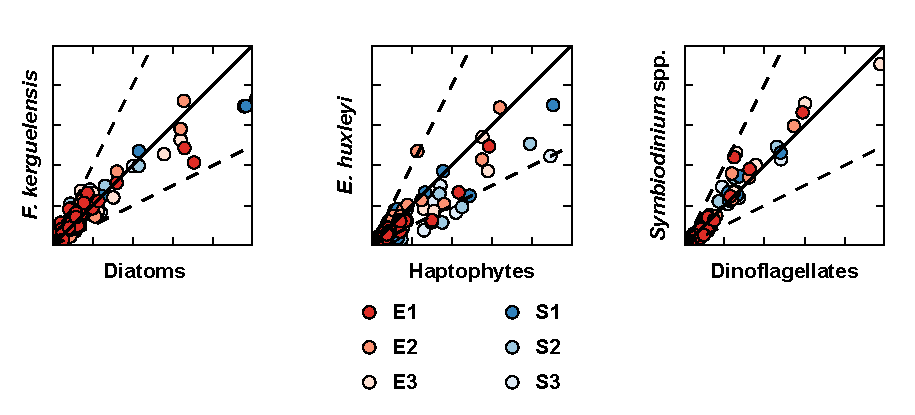
\includegraphics[width=1\textwidth]{Images/C4_FigureS3.pdf}
    \caption[Comparison of the quantitative metabolic fingerprint (QMF) between the whole functional group and representative taxa]{Comparison of the quantitative metabolic fingerprint (QMF) between the whole functional group and representative taxa. The proportion of reads falling into each of the modules depicted in Figure 2 is plotted for S1-S3 and E1-E3, comparing the summed functional group signal and that of a representative taxon. Color of the marker indicates the sample; solid and dashed lines mark the 1:1 and 1:2 lines, respectively.}
  \label{fig:a4f3}
\end{figure}

%Supplemental Figure 4: Distribution histogram

\begin{figure}[p!]
  \centering
    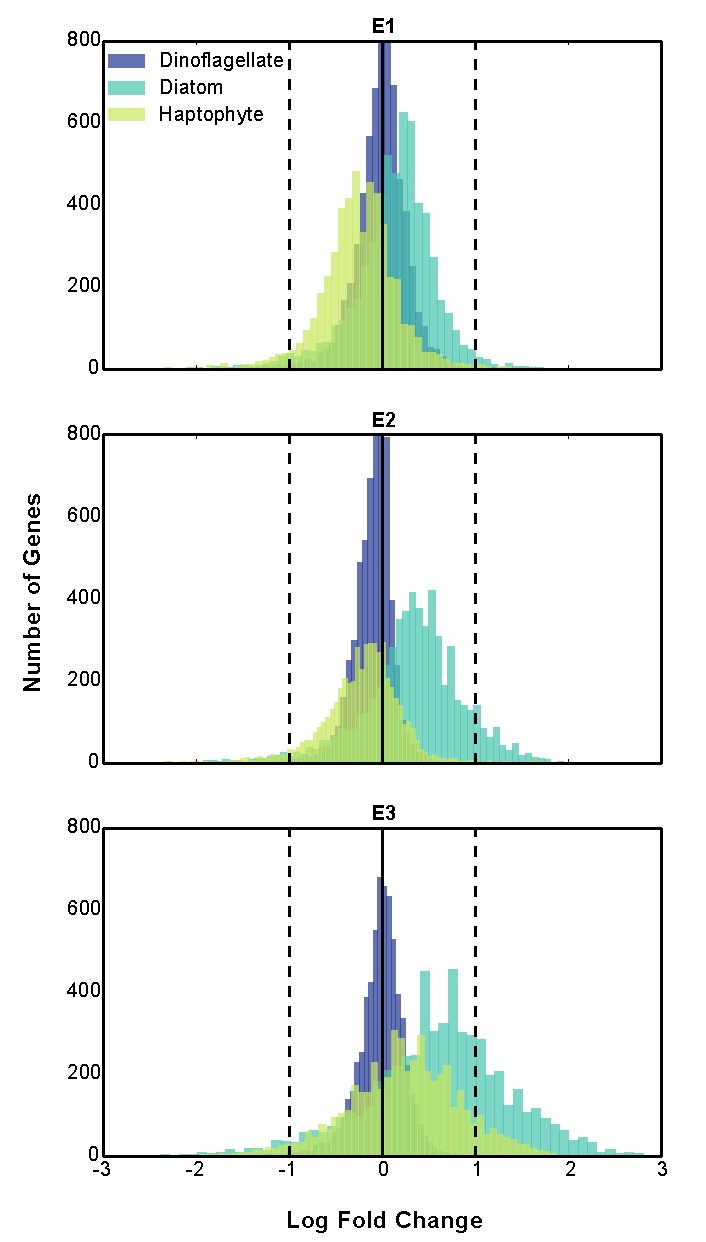
\includegraphics[width=.75\textwidth]{Images/C4_FigureS4.png}
    \caption[Distribution of log fold change following deep seawater (DSW) addition]{Distribution of log fold change following deep seawater (DSW) addition. Histogram of the number of genes falling within each of the log fold change bins for diatoms, haptophytes and dinoflagellates. Solid line indicates no fold change; dashed lines indicate 2 fold-change both up and down.}
  \label{fig:a4f4}
\end{figure}


%Supplemental Figure 5: Weight venn diagrams for up and down regulated genes

\begin{figure}[p!]
  \centering
    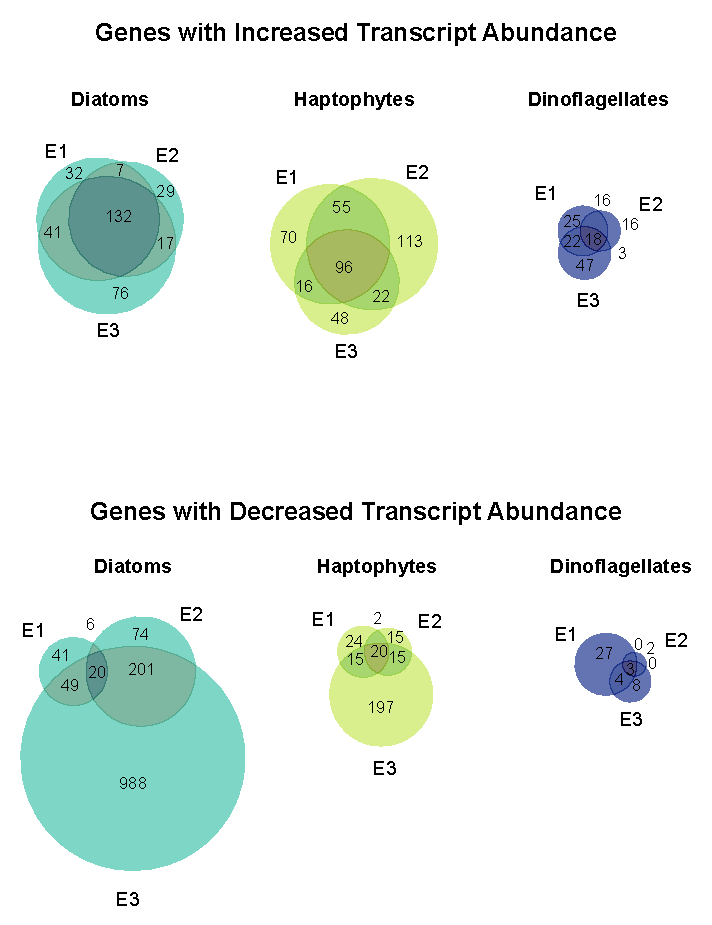
\includegraphics[width=1\textwidth]{Images/C4_FigureS5.pdf}
    \caption[Weighted Venn diagrams of genes with significantly different abundances following deep seawater (DSW) addition by functional group]{Weighted Venn diagrams of genes with significantly different abundances following deep seawater (DSW) addition by functional group. The uniqueness of KEGG orthologs with increased or decreased abundances as determined by ASC (2 fold-change, post-p > 0.95) across experiments was assessed for diatoms, haptophytes, and dinoflagellates.}
  \label{fig:a4f5}
\end{figure}


%Supplemental Figure 6: MANTA Plots

\begin{figure}[p!]
  \centering
    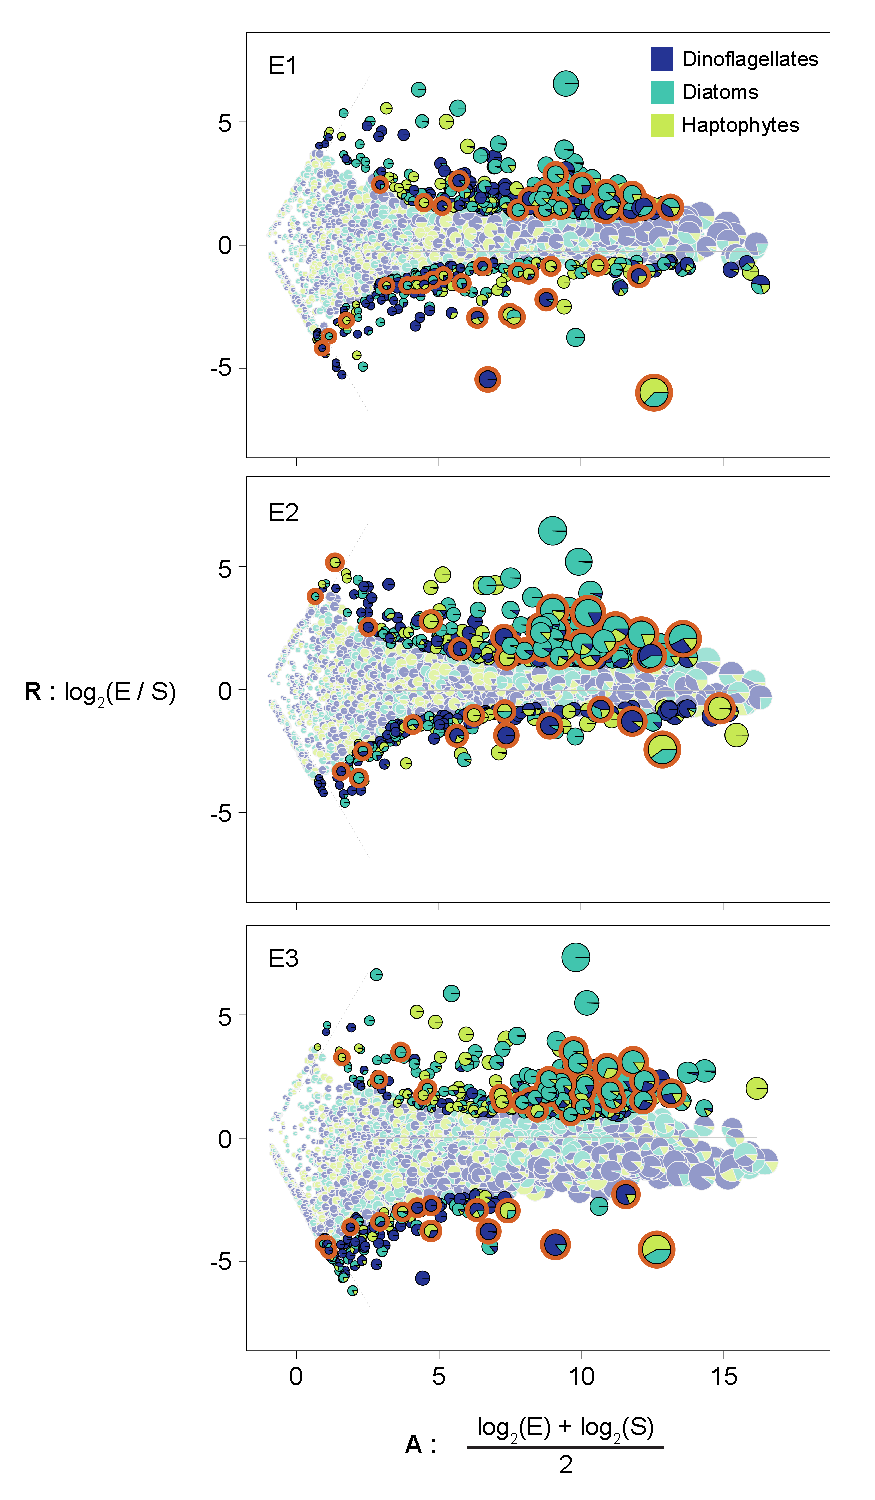
\includegraphics[width=.7\textwidth]{Images/C4_FigureS6.pdf}
    \caption[Microbial Assemblage Normalized Transcript Analysis (MANTA) ratio-averaged plots for global shifts in expression of KEGG orthologs]{Microbial Assemblage Normalized Transcript Analysis (MANTA) ratio-averaged plots for global shifts in expression of KEGG orthologs. Fold change ratio (R) and average read count (A) are plotted for read counts in the \emph{in situ} (S) and deep seawater (DSW) amendment (E) samples across the three sample pairs (S1:E1, S2:E2, S3:E3). The trimmed mean of fold-change values is noted as a gray solid line; orthologs unique to one library are separated by gray dashed lines. Pies indicate the taxonomic distribution of orthologous reads across the three functional groups. KEGG orthologs that were significantly differentially expressed (DE) (adjusted $P > 0.05$) are outlined in black and those not significantly DE are outlined in gray. DE KEGG orthologs that fall in the Energy Metabolism KEGG module are outlined in orange.}
  \label{fig:a4f6}
\end{figure}

%Supplemental Figure 7: QMF across incubation experiments

\begin{figure}[p!]
  \centering
    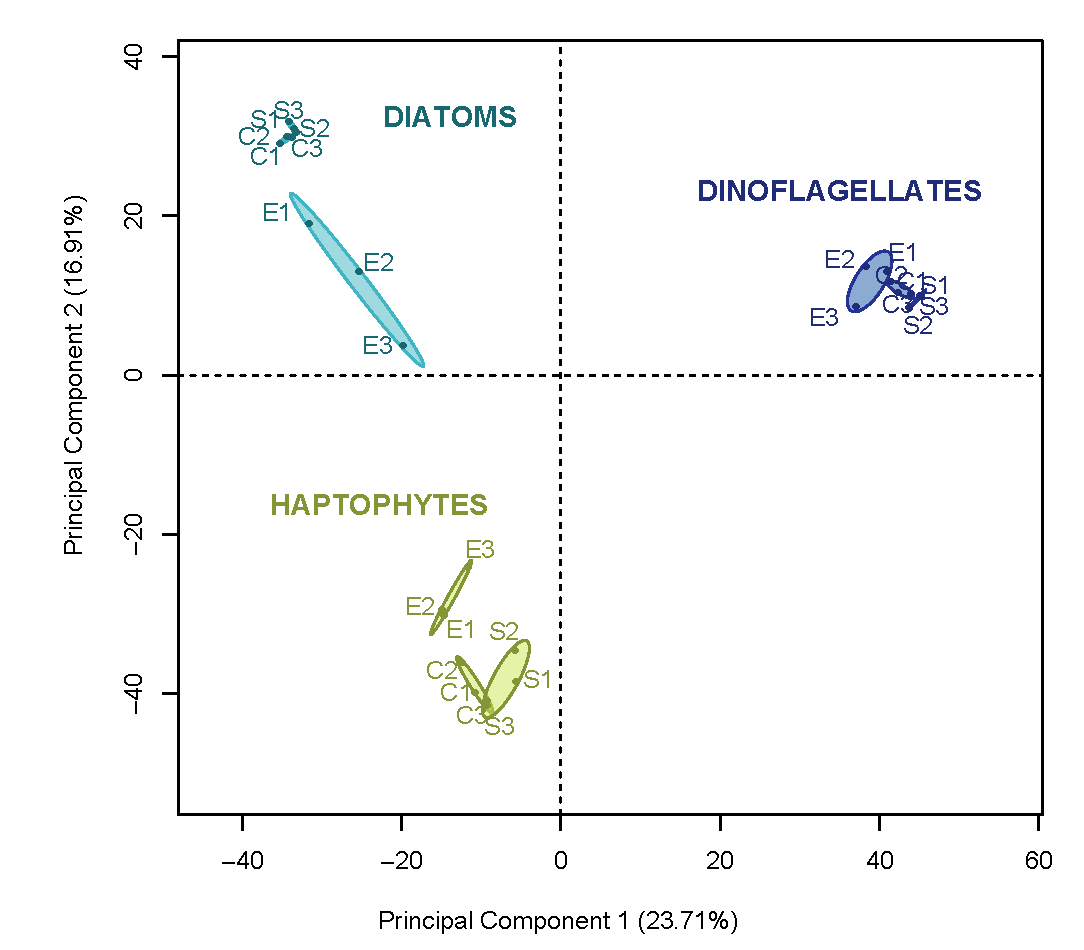
\includegraphics[width=1\textwidth]{Images/C4_FigureS7.pdf}
    \caption[Principal component analysis of the quantitative metabolic fingerprint (QMF) signals across \emph{in situ}, no addition control, and deep seawater amended samples]{Principal component analysis of the quantitative metabolic fingerprint (QMF) signals across \emph{in situ}, no addition control, and deep seawater (DSW) amended samples. Principal component analysis of the QMF signals for each of the functional groups across \emph{in situ} (S1-S3), control no addition (C1-C3) and DSW amendment (E1-E3); 95\% confidence ellipses are indicated for each of the sample types by functional group.}
  \label{fig:a4f7}
\end{figure}

\clearpage

\section{Supplemental Tables}

% Supplemental table with nutrient concentrations post treatment run for E and C
\begin{table}[h!]
\centering
\caption[Macronutrient concentrations in deep seawater ammendment and the incubation experiments after 168 hours]{Macronutrient concentrations in control no addition (C), DSW-amended incubations (E), and 700 m water used in DSW amendment incubations}
\label{tab:a4t1}
\newcolumntype{C}[1]{>{\centering\let\newline\\\arraybackslash\hspace{.5pt}}m{#1}}
\begin{tabular}{ccccc}

    
\hline
\multicolumn{1}{|c|}{\multirow{2}{*}{\textbf{Treatment}}} & \multicolumn{1}{c|}{\multirow{2}{*}{\textbf{\begin{tabular}[c]{@{}c@{}}Time post \\ inoculation (hours)\end{tabular}}}} & \multicolumn{1}{c|}{\multirow{2}{*}{\textbf{\begin{tabular}[c]{@{}c@{}}NO$_2$ + NO$_3$ \\ ($\mu M$)\end{tabular}}}} & \multicolumn{1}{c|}{\multirow{2}{*}{\textbf{\begin{tabular}[c]{@{}c@{}}PO$_4$ \\ ($\mu M$)\end{tabular}}}} & \multicolumn{1}{c|}{\multirow{2}{*}{\textbf{\begin{tabular}[c]{@{}c@{}}Si\\ ($\mu M$)\end{tabular}}}} \\

\multicolumn{1}{|c|}{}                                    & \multicolumn{1}{c|}{}                                                        & \multicolumn{1}{c|}{}                                                                                    & \multicolumn{1}{c|}{}                                                                              & \multicolumn{1}{c|}{}                                                                            \\ \hline
\multicolumn{1}{|c|}{\textbf{C} (control no addition) *}  & \multicolumn{1}{c|}{168}                                                     & \multicolumn{1}{c|}{$0.12 \pm 0.03$}                                                                         & \multicolumn{1}{c|}{$0.12 \pm 0.02$}                                                                   & \multicolumn{1}{c|}{$1.91 \pm 0.2$}                                                                  \\ \hline
\multicolumn{1}{|c|}{\textbf{E} (+ 10\% DSW) *}           & \multicolumn{1}{c|}{168}                                                     & \multicolumn{1}{c|}{$1.9 \pm  .93$}                                                                          & \multicolumn{1}{c|}{$0.23 \pm 0.05$}                                                                   & \multicolumn{1}{c|}{$8.46 \pm 3.11$}                                                                 \\ \hline
\multicolumn{1}{|c|}{\textbf{DSW} (700 m water) *}        & \multicolumn{1}{c|}{N/A}                                                     & \multicolumn{1}{c|}{$37.5 \pm 1.68$}                                                                         & \multicolumn{1}{c|}{$3.14 \pm 0.03$}                                                                   & \multicolumn{1}{c|}{$83.4 \pm 9.33$}                                                                 \\ \hline
\multicolumn{5}{l}{\textit{* Nutrient data averaged for E1 and E2, nutrients were not assayed on E3.}}                                                                                                                                                                                                                                                                                                                                                     
\end{tabular}
\end{table}

